\chapter{Continuity}
Assume general metric spaces $X,Y$ and $f: X\to Y$.
\begin{definition}[Definition 4.1]
	\label{def:4.1}
	Suppose $X,Y$ are metric spaces, $E \subset X$, $f: E\to Y$, $p \in E'$, where $E'$: set of limit points in metric space $X$.
	We say $\lim_{x\to p}{f(x)}=q$, or $f(x)\to q$ as $x\to p$, if $\forall_{\epsilon > 0}: \exists_{\delta>0} \text{ s.t. } (0<d_X(x,p)<\delta \text{ and } x \in E) \implies d_Y(f(x),q)<\epsilon $.
	\begin{note}
		We don't say anything about $x=p$, $f(p)$ may not even be defined.
	\end{note}
\end{definition}

% \begin{example}
% Note that we require $x$ to be in $E$.
% For instance, let the next figure represent $E \subset X$.
% \end{example}

\begin{theorem}[2]
	$\lim_{x\to p}{f(x)}=q \Leftrightarrow \forall_{\{ {p}_{n}\} \text{ in } E}: \lim_{n\to \infty}{f(p_{n})}=q$ such that $p_{n}=p$ and $p_{n}\to p$, where the RHS is the limit of Definition 3.1.
	\begin{note}
		This implies uniqueness of $q$ in Definition 4.1.
	\end{note}
	\begin{proof}
		\begin{description}
			\item[$\implies $]
			      Suppose $\lim_{x\to p}{f(x)}=q$. Let $\epsilon>0$. Choose $\delta>0$ s.t. $d_Y(f(x),q)\epsilon$ if $0<d_X(x,p)<\delta$.
			      Let $\{ p_{n} \}$ be a sequence in $E$ such that $p_{n}\to p$ and $p_{n}\neq p$. Then $\exists_{N} \text{ s.t. } 0<d_X(p_{n},p)<\delta $ if $n\ge N$; i.e., $f(p_n)\to q$.
			\item[$\impliedby$]
			      Consider the contrapositive of $(\impliedby) $: $\neg(\lim_{x\to p}{f(x)}=q) \implies \neg(\forall_{\{ p_{n} \} \text{ in } E}: \lim_{n\to \infty}{f(p_{n})}=q)$.
			      Suppose $\neg(\lim_{x\to p}{f(x)}=q)$. Then $\exists_{\epsilon>0} \text{ s.t. } \forall_{\delta>0}: \exists_{x\in N_{\delta}^{E}(p)} \text{ s.t. } x\neq p \text{ and } d_Y(f(x),q)\ge \epsilon$.
			      Take $\delta=\delta_n=\frac{1}{n}$ and let $p_{n}$ be an $x$ as above for $\delta_n$. Then $p_{n}\to p$, but $d_Y(f(p_{n}),q)\ge \epsilon \forall n$, so $f(p_{n})\not \to q$.
		\end{description}
	\end{proof}
\end{theorem}

\begin{theorem}[4]
	When $Y=\C$, limit as defined in Definition~\ref{def:4.1} respects sums, products and quotients.
	\begin{proof}
		By Theorem~\ref{thm:4.2}, it suffices to show that the theorem holds for sequences.
	\end{proof}
\end{theorem}

\begin{definition}
	\label{def:4.5}
	Suppose $X,Y$ are metric spaces, $p \in E \subset X$, $f: E\to Y$. Then $f$ is continuous at $p$ if $\forall_{\epsilon > 0}: \exists_{\delta > 0} \text{ s.t. } d_X(x,p)<\delta \implies d_Y(f(x),f(p))<\epsilon$; i.e., $f(N_{\delta}^{E}(p)) \subset N_{\epsilon}^{y}(f(p))$. We say $f$ is continuous if $f$ is continuous at $p$ for all $p \in E$.
	\begin{note}
		If $p$ is an isolated point; i.e., $\exists_{\delta >0} \text{ s.t. } N_{\delta}^{E}(p)=\{p\}$, then every $f: E\to Y$ is continuous at $p$.
	\end{note}
\end{definition}

\begin{theorem}[6]
	Suppose $E \subset X, p \in E \cap E', f: E\to Y$. Then $f$ is continuous at $p$ if and only if $\lim_{x\to p}{f(x)}=f(p)$.
	\begin{proof}
		By Definition~\ref{def:4.1} and Definition~\ref{def:4.5} with $q=f(p)$.
	\end{proof}
\end{theorem}

\begin{theorem}[7]
	For $E \subset  X, f: E\to Y, g: f(E)\to Z$, let $h=g \circ f: E\to Z$. If $f$ is continuous at $p \in E$ and if $g$ is continuous at $f(p) \in Y$, then $h$ is continuous at $p$.
	\begin{proof}
		Choose $\eta>0$ such that $d_{Y}(f(p),y)<\eta \implies d_{Z}(g(f(p)),g(y))<\epsilon$ (continuity of $g$ at $f(p)$).
		Choose $\delta>0$ s.t. $d_E(x,p)<\delta \implies d_Y(f(x),f(p))<\eta$ (continuity of $f$ at $p$).
		Then $d_E(x,p)<\delta \implies d_Z(g(f(x)),g(f(p)))=d_Z(h(x),h(p))<\epsilon$.
	\end{proof}
	% \begin{note}
	% Proof is essentially the following diagram:
	% \begin{center}
	% \begin{tikzcd}
	% 	E \arrow[r, "f"] \arrow[rd, "h=g\circ f"'] & f(E) \arrow[d, "g"] \\
	% 	& Z
	% \end{tikzcd}
	% \end{center}
	% \end{note}
\end{theorem}

\begin{theorem}[8][Theorem 4.8: Topological Characterization of Continutiy]
	$f: X\to Y$ is continuous $\Leftrightarrow  f^{-1}(V)$ is open for every open $V \subset Y$.
	\begin{proof}
		\begin{description}
			\item[$(\implies)$]
			      Suppose $f$ is continuous. Let $V \subset Y$ be open. Then $f^{-1}(V)$ is open.
			      Let $p \in f^{-1}(V)$. We need to show {$\exists_{\delta >0} \text{ s.t. } \linebreak N_{\delta}^{X}(p) \subset f^{-1}(V)$.} Since $V$ is open, $\exists_{\epsilon > 0} \text{ s.t. } N_{\epsilon}^{Y}(f(p)) \subset V$.
			      Since $f$ is continuous, $\exists_{\delta > 0} \text{ s.t. } f(N_{\delta}^{X}(p)) \subset N_{\epsilon}^{Y}(f(p)) \subset V$.
			      % 	  Then $f(p) \in V$. Since $V$ is open, $\exists_{\epsilon>0} \text{ s.t. } N_{\epsilon}^{Y}(f(p)) \subset V$.
			      %       Since $f$ is continuous at $p$, $\exists_{\delta>0} \text{ s.t. } f(N_{\delta}^{X}(p)) \subset N_{\epsilon}^{Y}(f(p)) \subset V$.
			      %       Thus, $N_{\delta}^{X}(p) \subset f^{-1}(V)$, so $f^{-1}(V)$ is open.
			\item[$(\impliedby)$]
			      Suppose $f^{-1}(V)$ is open for every open $V \subset Y$. Let $p \in X$ and $\epsilon>0$. Then $N_{\epsilon}^{Y}(f(p))$ is open, so $f^{-1}(N_{\epsilon}^{Y}(f(p)))$ is open. Take $V=N_{\epsilon}^{Y}(f(p))$, which is open.
			      Since $f^{-1}(V)$ is open and $p \in f^{-1}(V)$, there exists $\delta>0$ such that $N_{\delta}^{X}(p) \subset f^{-1}(V)$. Then $f(N_{\delta}^{X}(p)) \subset V=N_{\epsilon}^{Y}(f(p))$; i.e., $f$ is continuous at $p$.
		\end{description}
	\end{proof}
	\begin{remark}\hfill
		\begin{enumerate}
			\item
			      \hfill\\
			      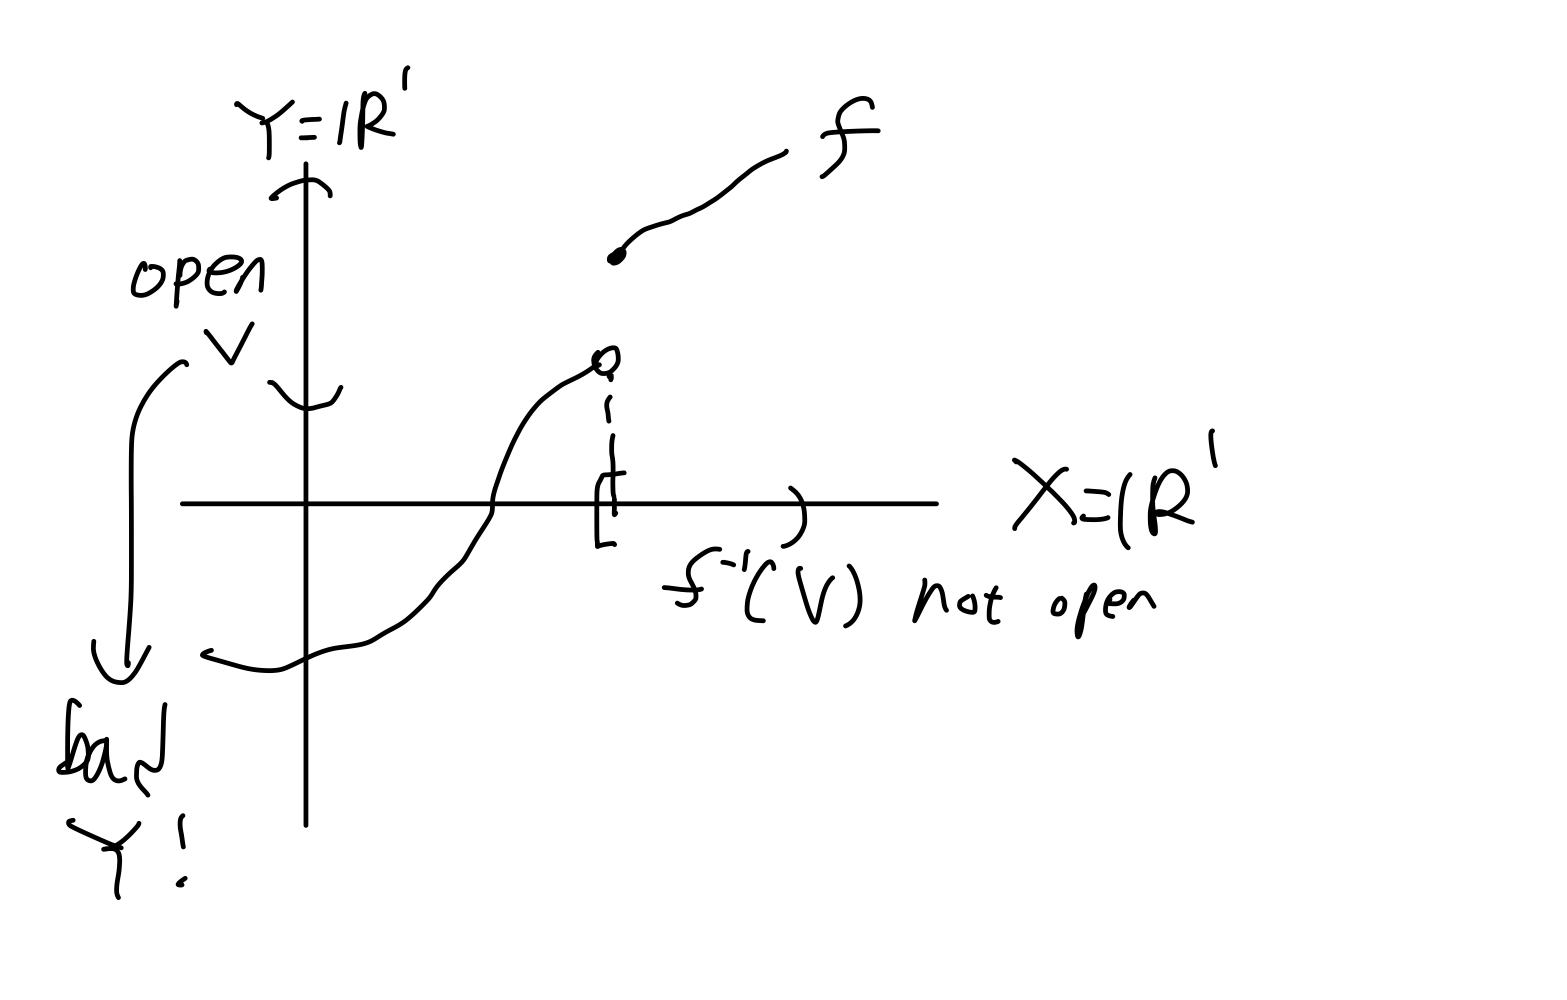
\includegraphics[width=0.5\textwidth]{./figs/thm4-8-a.jpeg}
			\item Continuity is determined by the open sets, not the metric. For instance, if metrics $l_1,l_2,l_{\infty}$ have the same open sets in $\R^{k}$, hence the same continuous functions.
			      \[
				      l_1(x,y)=\sum_{i=1}^{k}{|x_i-y_i|}
			      \]
			      \[
				      l_2(x,y)=\sqrt{\sum_{i=1}^{k}{(x_i-y_i)^2}}
			      \]
			      \[
				      l_{\infty}(x,y)=\max_{1\le i\le k}{|x_i-y_i|}
			      \]
			\item $f$ with open $U \subset X \implies f(U)$ is open are called open maps. Continuous maps need not be open(e.g., $f(x)=\text{some constant}$, $f(x)=x^2$), and open maps need not be continuous(e.g., floor function: $\left\lfloor \cdot \right\rfloor: \R\to \Z$).
		\end{enumerate}
	\end{remark}
\end{theorem}

\begin{corollary}
	$f:X\to Y$ is continuous if and only if $f^{-1}(F)$ is closed for every closed $F \subset Y$.
	\begin{proof}
		Let $V \subset Y$ be open and $F=V^{c}$. Then the above condition (RHS) is the same as $f^{-1}(V)=f^{-1}(F^{c})=(f^{-1}(F))^{c}$ is open.
	\end{proof}
\end{corollary}


\begin{theorem}[9]
	Let $f: X\to \C, g: X\to \C$ be continuous. Then $f+g, f \cdot g, f/g(\text{at points $p$ where $g(p)\neq 0$})$ are also continuous.
\end{theorem}

\begin{theorem}[10]
	Given $f_i: X\to \R(i=1,2,\ldots ,k)$, define $f: X\to \R^{k}$ by $f(x)=(f_1(x),\ldots ,f_k(x))$.
	Then
	\begin{enumerate}
		\item
		      $f$ is continuous if and only if each $f_i$ is continuous.
		\item if $f,g: X\to \R^{k}$ are continuous, then so are $f+g: X\to \R^{k}, f \cdot g: X\to \R^{1}$
	\end{enumerate}
\end{theorem}


\begin{example}
	\label{eg:4.11}
	\begin{enumerate}
		\item For $i=1,\ldots ,k$, define $\phi_i: \R^{k}\to \R$ by $\phi_i(x)=x_i$, where $x=(x_1,x_2,\ldots ,x_k)$. Then $|\phi_{i}(x)-\phi_{i}(y)|=|x_i-y_i|\le \left( \sum_{j=1}^{k}{|x_j-y_j|^{2}} \right)^{1/2}=|x-y|$, so $\phi_{i}$ is continuous(take $\delta=\epsilon$. If $|x-y|<\delta=\epsilon$, then $|\phi_{i}(x)-\phi_{i}(y)|<\epsilon$).
		\item The functions $\R^{k}\to \R$ defined by $x \mapsto x_1^{n_1}x_2^{n_2}\cdots x_k^{n_k}(n_i \in \{0,1,2,\ldots \})$ is continuous on $\R^{k}$ and so is any polynomial $P(x)=\sum{C_{n_1,n_2,n_3,\ldots ,n_k}x_1^{n_1} x_2^{n_2}\cdots x_k^{n_k}}$, where $C_{n_1,n_2,n_3,\ldots ,n_k}$ is a constant (function) in $\C$.
		\item Rational functions $f(x)=\frac{P(x)}{Q(x)}$ are continuous at points where $Q(x)\neq 0$.
		\item The function $\R^{k} \to \R$ defined by $x \mapsto |x|$ is continuous.
		      \begin{proof}
			      $|x|=|y+(x-y)|\le |y|+|x-y|$, so $|x|-|y|\le |x-y|$. Similarly, $|y|-|x|\le |y-x|$, so $||x|-|y||\le |x-y|$. Thus by taking $\delta=\epsilon$, $|x-y|<\delta \implies ||x|-|y||<\epsilon$.
		      \end{proof}
		\item Suppose $f: X\to \R^{k}$ is continuous. Then $p \mapsto |f(p)|$ is continuous.
		      \begin{proof}
			      $p \mapsto |f(p)|= (y \mapsto |y|) \circ (p \mapsto f(p))$.
			      Since both $(y \mapsto |y|)$, $(p \mapsto f(p))$ are continuous, $p \mapsto |f(p)|$ is continuous by Theorem~\ref{thm:4.7}.
		      \end{proof}
	\end{enumerate}
\end{example}
\begin{note}
	A function is said to be continuous on the \textit{domain}, not on the \textit{range}.
\end{note}

\begin{theorem}[14]
	Let $f: X\to Y$ be continuous and $X$ be compact. Then $f(X)$ is compact.
	\begin{proof}
		Let $\{ V_{\alpha} \}$ be an open cover of $f(X)$.
		We need to find a finite subcover of $f(X)$.
		By Theorem~\ref{thm:4.8}, each set $O_{\alpha}=f^{-1}(V_{\alpha})$ is open and $\bigcup_{\alpha} O_{\alpha}=\bigcup_{\alpha} f^{-1}(V_{\alpha})=f^{-1}(\bigcup_{\alpha}V_{\alpha})=f^{-1}(f(X))=X$. Hence, $\{O_{\alpha}\} $ is an open cover of $X$, so there exists a finite subcover $X=O_{\alpha_1} \cup \cdots \cup O_{\alpha_n}$.
		However, then $f(x)=\bigcup_{i=1}^{n}f(O_{\alpha_{i}})= \bigcup_{i=1}^{n}f(f^{-1}(V_{\alpha_{i}})) \subset \bigcup_{i=1}^{n}V_{\alpha_i}$. Therefore, $\{V_{\alpha_{i}}\}^{n}_{i=1}$ is a finite subcover of $f(X)$.
	\end{proof}
\end{theorem}
\begin{definition}[4.13]
	\label{def:4.13}
	$f: E \to \R^{k}$ is bounded if $\exists_{M>0} \text{ s.t. } |f(x)|\le M\, \forall x \in E$.
\end{definition}

\begin{theorem}[15]
	If $X$ is compact and $f:X\to \R^{k}$, then $f(X)$ is closed and bounded (so $f$ is bounded).
	\begin{proof}
		$f(X)$ is compact by Theorem~\ref{thm:4.14}, and since $f(X) \subset \R^{k}$, it is closed and bounded.
	\end{proof}
\end{theorem}

\begin{thm}[16]
	If $X$ is compact and $f:X\to \R^{1}$ is continuous, then $\exists_{p,q \in X}\text{ s.t. } f(p)\le f(x)\le f(q)$ for all $x \in X$.
	\begin{proof}
		By Theorem~\ref{thm:4.15}, $f(X)$ is closed and bounded.
		% By Theorem~\ref{thm:2.28}, $M \in f(X)$ and similarly $m \in f(X)$.
		By Theorem 2.28, $M \in f(X)$ and similarly $m \in f(X)$.
	\end{proof}
\end{thm}
\begin{example}
	Let $X=(0,1)$, not compact, let $f(x)=\frac{1}{x}$, continuous. However, $\nexists_{p \in X} \text{ s.t. } \forall_{x \in X}:  f(p)\le f(x)$ and $\not \exists_{q \in X} \text{ s.t. } \forall_{x \in X}:  f(x)\le f(q)$.
\end{example}


\begin{theorem}[17]
	Suppose $f:X\to Y$ is one-to-one, onto, continuous, where $X$ is compact.
	Define $f^{-1}: Y\to X$ by $f^{-1}(f(x))=x$. Then $f^{-1}$ is continuous.
	\begin{proof}
		By Theorem~\ref{thm:4.8}, it suffices to prove that if $V \subset X$ is open then $(f^{-1})^{-1}(v)(=f(v))$ is open. However, $V^{c} \subset X$ is closed, hence $V^{c}$ is compact by Theorem~\ref{thm:4.14} and $(f(V^{c}))^{c}=f(V)$ is open.
	\end{proof}
\end{theorem}
\begin{example}[Compactness is needed in Theorem~\ref{thm:4.17}]
	Let $X=[0,2\pi), Y=\{(x,y) \in \R^{2}: x^2+y^2=1\}$. Define $f:X\to Y$ by $f(\theta)=(\cos{\theta},\sin{\theta})$.
	This $f$ is 1-1, onto, and continuous, but $f^{-1}$ is not continuous as $X$ is not compact.
	\begin{proof}
		\begin{enumerate}[label=(\arabic*)]
			\item $[0,1) \subset X$ is open but $(f^{-1})^{-1}([0,1))=f([0,1))$ is not open because $(1,0)$ is not an interior point of $Y$.
			\item In $Y$, as $(x,y)\to (1,0)$ from above, $f((x,y))\to 0$.
			      As $(x,y)\to (1,0)$ from below, $\lim{f^{-1}(x,y)}$ does not exist in $X$. (Wants to be $2\pi \not\in X$), so $f^{-1}$ is not continuous at $(1,0) \in Y$.
		\end{enumerate}
	\end{proof}
\end{example}

\begin{define}[18]
	Let $X,Y$ be metric spaces and $f:X\to Y$.
	$f$ is uniformly continuous on $X$ if $\forall_{\epsilon > 0}: \exists_{\delta > 0} \text{ s.t. } \text{ for all } p,q \in X$ with $d_x(p,q)<\delta$, we have $d_Y(f(p),f(q))<\epsilon$.
	\begin{remark}
		The point is for any $\epsilon$, there is some $\delta$ that works for every $p,q \in X$ such that $d(p,q)$.
	\end{remark}
\end{define}

\begin{example}
	\begin{enumerate}
		\item $X=(0,1), Y=\R,f(x)=\frac{1}{x}$. $f$ is continuous on $X$ but is not uniformly continuous.
		      \begin{proof}
			      For $x \in (0,\frac{1}{2})$, $|f(x)-f(2x)|=|\frac{1}{x}-\frac{1}{2x}|=\frac{1}{2x}\to \infty$ as $x \to 0$. Then $\text{ for } \epsilon=1$, given any $\delta \in (0,\frac{1}{2})$, we can pick $x<\delta$ s.t. $d_(X)(x,2x)=x<\delta$, but $d_Y(f(x),f(2x))=\frac{1}{2x}>\frac{1}{2 \delta}>1$.
		      \end{proof}
		\item $X=[0,5], Y=\R,f(x)=x^2$ is uniformly continuous.
		      \begin{proof}
			      For $0\le x_1\le x_2\le 5$ and $\epsilon>0$, $|f(x_1)-f(x_2)|=x_2^2-x_1^2=(x_2-x_1)(x_2+x_1)\le 10 \cdot (x_2-x_1)$, which is less than $\epsilon$ if $|x_2-x_1|<\frac{\epsilon}{10}=\delta$
		      \end{proof}
	\end{enumerate}
\end{example}

\begin{theorem}[19]
	Suppose $X$ is a compact metric space, $Y$ is a metric space, and $f:X\to Y$ is continuous. Then $f$ is uniformly continuous.
	\begin{proof}
		Fix $\epsilon>0$. For $p \in X$ there exists $\delta=\delta_p(\epsilon)$ s.t. $d_{X}(p,q)<\delta_{p}\implies d_Y(f(p),f(q))<\frac{\epsilon}{2}$.
		We need to remove the $p$-dependence of $\delta_p$.
		Let $J_{p}=N_{\frac{1}{2}\delta_{p}}(p)$. Then $\{ {J}_{p}\}_{p \in X}$ is an open cover of $X$.
		Then there exists subcover $X= J_{p_1} \cup J_{p_2}\cdots \cup J_{p_n}$ (equality works as $X$ is the whole metric space, so $X \subset J \implies X=J$).
		Let $\delta=\min\{\frac{1}{2}\delta_{p_1},\frac{1}{2}\delta_{p_2},\ldots ,\frac{1}{2}\delta_{p_n}\}$.
		Suppose $p,q$ with $d_{X}(p,q)<\delta$. Choose $m \in \{1,2,\ldots n\}$ s.t. $p \in J_{p_m}$. Then $d_{X}(p,p_{n})<\frac{1}{2}\delta_{p_{m}}$.
		$d_X(q,p_{m})\le d_X(q,p)+d_{X}(p,p_{m})<\delta+\frac{1}{2}\delta p_{m}\le \delta p_m$.
		$\therefore d_Y(f(q),f(p))\le d_Y(f(q),f(p_{m}))+d_Y(f(q_m),f(p))<\frac{\epsilon}{2}+\frac{\epsilon}{2}=\epsilon$.
	\end{proof}
\end{theorem}

\begin{theorem}[22]
	If $X,Y$ are metric spaces, $f:X\to Y$ is continuous, and $E \subset X$ is connected, then $f(E)$ is connected.
	\begin{proof}[By Contradiction]
		Suppose for contradiction $E$ is connected and there exists $A,B \subset Y$ s.t. $f(E)=A \cap  B$, $f(E) \neq \emptyset$, $\overline{A} \cup B=A \cap \overline{B}=\emptyset$.
		Let $G=f^{-1}(A) \cap E, H=f^{-1}(B)\cap E$. Then $E=G \cup H$, $G,H$ are nonempty.
		If $G \cap \overline{H}=\overline{G} \cap H=\emptyset$, it leads to a contradiction.
		First, $G \subset f^{-1}(A) \subset(\because A \subset \overline{A}) f^{-1}(\overline{A})$, where $f^{-1}(\overline{A})$ is closed by the corollary to Theorem~\ref{thm:4.8}, so $\overline{G} \subset f^{-1}(\overline{A})$.
		Second, $f(H)=B, \overline{A} \cap B=\emptyset$.
		Therefore, $\overline{G} \cap H =\emptyset$.
		WLOG, $G \cap \overline{H} = \emptyset$ as well.
		Hence a contradiction.
	\end{proof}
\end{theorem}

\begin{theorem}[23][Intermediate Value Theorem]
	Suppose $f: [a,b]\to \R$ is continuous. If $f(a)<f(b) \text{ and } c \in (f(a),f(b))$. Then $\exists_{x_0 \in (a,b)} \text{ s.t. } f(x_0)=c$.
	\begin{proof}
		$[a,b]$ is connected by Theorem~\ref{thm:2.47}. Hence, by Theorem~\ref{thm:4.22}, $f([a,b])$ is connected and therefore contains all points between $f(a)$ and $f(b)$. In particular, $c \in f((a,b))$
	\end{proof}
\end{theorem}

\begin{example}
	\begin{enumerate}
		\item there exists a continuous function called (Peano/space-filling curve) from $[0,1]$ onto the closed unit square $S=[0,1]\times [0,1] \subset \R^2$.
		      \begin{proof}
			      See Rudin, problem $7.14$ for an explicit example(covered in MATH-321).
		      \end{proof}
		\item But no such function can be one-to-one.
		      \begin{proof}

		      \end{proof}
	\end{enumerate}
\end{example}
